\documentclass[11pt,a4paper]{article}

% ---------- Packages ----------
\usepackage[T1]{fontenc}
\usepackage[utf8]{inputenc}
\usepackage{lmodern}
\usepackage[margin=2.5cm]{geometry}
\usepackage{microtype}
\usepackage{amsmath}
\usepackage{booktabs}
\usepackage{tabularx}
\usepackage{array}
\usepackage{enumitem}
\usepackage{xcolor}
\usepackage{pgfplots}
\pgfplotsset{compat=1.17}
\usepackage[font=small,labelfont=bf]{caption}
\usepackage[numbers,sort&compress]{natbib}
\usepackage[colorlinks=true,linkcolor=blue!50!black,citecolor=blue!50!black,urlcolor=blue!50!black]{hyperref}

\definecolor{compblue}{RGB}{31,111,201}
\definecolor{othergray}{RGB}{185,185,185}
\setlist{itemsep=2pt,topsep=4pt}
\newcolumntype{L}{>{\raggedright\arraybackslash}X}

% ---------- Title ----------
\title{\textbf{How AI Agents Treat Each Other:}\\[2pt]
\Large An Axelrod-Style Iterated Prisoner's Dilemma\\ Tournament with Language-Model Agents\\[4pt]
\large A Pilot Study}
\author{[Your Name]\\ \small Independent Researcher}
\date{October 2026}

\begin{document}
\maketitle

\begin{abstract}
\noindent
As autonomous AI agents begin to act on behalf of people online, they will increasingly interact with one another in repeated encounters where cooperation and exploitation are both possible. We study this setting with an Axelrod-style iterated Prisoner's Dilemma tournament in which large language model (LLM) agents of three sizes compete alongside three fixed-strategy bots. The game includes execution noise (10\%), optional non-binding messages, and a public reputation signal. Agents were assigned one of three goal framings: neutral (maximise total points), cooperative (maximise points while valuing fairness), or competitive (``beat your opponents'' in each match). Across 20 tournaments in four settings, neutral and cooperative agents almost never defected first and forgave most noise-induced defections. The competitive framing produced two qualitatively different strategies: a cooperate-then-betray strategy accompanied by friendly messages, which won its setting, and unconditional defection, which won most head-to-head matches yet finished 7th or 8th of 8, reproducing Axelrod's observation that envious strategies lose. Goal wording affected behaviour more than model size, no agent was persuaded by a lying bot, and a single aggressive player lowered every other player's score. A follow-up check revealed that batching several games into one model call makes games non-independent, which weakens one of our comparisons. We discuss implications for multi-agent AI systems and outline a larger confirmatory study.
\end{abstract}

\section{Introduction}

AI agents are beginning to act for people on the internet: buying, selling, negotiating and exchanging information. In many of these interactions, the counterpart will itself be an AI agent, and the same agents will meet repeatedly. Whether such agents cooperate or exploit one another will shape the norms of this emerging ``agent internet''.

The iterated Prisoner's Dilemma (IPD) is the canonical model of this tension. In a single round, defection dominates; yet when the game is repeated, conditional cooperation can be sustained. In his seminal computer tournaments, Axelrod \citep{axelrod1980,axelrod1984} found that the simple strategy \emph{Tit-for-Tat} (cooperate first, then copy the opponent's previous move) performed best. He summarised successful strategies as \emph{nice} (never defect first), \emph{retaliatory}, \emph{forgiving}, and \emph{not envious}: a strategy that tries to beat each opponent, rather than to do well itself, tends to do poorly overall \citep{axelrod1981}.

This study replaces hand-coded strategies with LLM agents that read the game state in natural language and decide each move. We address four research questions:

\begin{enumerate}[label=\textbf{RQ\arabic*.}]
  \item Do LLM agents cooperate with one another, or exploit one another?
  \item Does the wording of an agent's goal change its behaviour?
  \item Does model size (small, medium, large) matter?
  \item Do non-binding messages (cheap talk) support cooperation or deception?
\end{enumerate}

\section{Method}

\subsection{Game}

Each tournament had eight players in a round-robin format: every player played a separate 10-round match against each of the other seven. Players were told that the tournament could end after any round and were not told its length. Payoffs followed Axelrod's standard values (Table~\ref{tab:payoff}).

\begin{table}[htbp]
\centering
\caption{Payoff matrix (row player's points, column player's points).}
\label{tab:payoff}
\begin{tabular}{lcc}
\toprule
 & Opponent: C & Opponent: D \\
\midrule
Player: C & (3, 3) & (0, 5) \\
Player: D & (5, 0) & (1, 1) \\
\bottomrule
\end{tabular}
\end{table}

\noindent Three further features made the environment closer to real agent interactions:
\begin{itemize}
  \item \textbf{Noise.} Each move was flipped with probability 0.10. Players saw their own intended and actual moves, but only their opponent's \emph{actual} moves, so accidental defections could not be told apart from deliberate ones.
  \item \textbf{Messages.} With each move, a player could send a message of at most 25 words, delivered at the start of the next round. Messages were non-binding and could be false.
  \item \textbf{Reputation.} Each player saw, for every opponent, the share of cooperative moves that opponent had played against \emph{other} players.
\end{itemize}
Player identities were hidden behind letters A--H, shuffled in every run.

\subsection{Players}

Each tournament contained five LLM agents and three fixed-strategy bots (Table~\ref{tab:players}). The small, medium and large agents were Claude Haiku, Sonnet and Opus models, respectively.

\begin{table}[htbp]
\centering
\caption{Players and their goals or rules.}
\label{tab:players}
\small
\begin{tabularx}{\textwidth}{@{}lL@{}}
\toprule
Player & Goal or rule \\
\midrule
Small, medium, large AI & \emph{Neutral}: ``earn as many total points as possible, summed across all of your matches.'' \\
Cooperative AI & Neutral goal, plus: ``you personally value fairness and mutual benefit.'' \\
Competitive AI & ``BEAT your opponents. In each match, try to finish with MORE points than that opponent.'' \\
\addlinespace
Tit-for-Tat bot & Cooperates first, then copies the opponent's previous actual move. \\
Random bot & Plays C or D with equal probability. \\
Cheat bot & Always defects. When messages are enabled it sends friendly lies (e.g.\ ``I always cooperate''). \\
Grudger bot & Cooperates until the opponent's first defection, then always defects (B2 only). \\
\bottomrule
\end{tabularx}
\end{table}

\subsection{Settings}

Four settings were run, five tournaments each (Table~\ref{tab:settings}). B1 and B2 reused the random seeds of S1, so seat assignments and noise draws were paired with S1.

\begin{table}[htbp]
\centering
\caption{Experimental settings (5 runs each).}
\label{tab:settings}
\small
\begin{tabular}{@{}lllll@{}}
\toprule
Setting & Competitive AI & Cooperative AI & Messages & Third bot \\
\midrule
S1 & Medium & Medium & On  & Lying cheat bot \\
S2 & Large  & Small  & On  & Lying cheat bot \\
B1 & Medium & Medium & Off & Silent cheat bot \\
B2 & Medium & Medium & Off & Grudger bot \\
\bottomrule
\end{tabular}
\end{table}

\subsection{Procedure}

In each round, every AI agent received a written prompt containing the rules, its goal, the full history of each of its matches, opponents' reputations and the latest messages. It returned a structured answer with one move per opponent, optional messages, and a brief rationale. Bot moves, noise and scores were computed by a game engine. All reported scores were recomputed from the raw move logs.

In a pilot run and in rounds 1--3 of S1, each agent was queried separately for each game. To reduce cost, later rounds used a single call per agent role that played the same seat in all parallel games of the round (5 games in S1 and S2; 10 in B1 and B2). Section~\ref{sec:check} shows that this design choice matters.

\subsection{Measures}

\begin{itemize}
  \item \textbf{Score:} total points over all matches, averaged over runs.
  \item \textbf{Cooperation rate:} share of intended moves that were C.
  \item \textbf{Unprovoked betrayal:} an intended D against an opponent whose actual moves in that match had all been C (matches against the cheat bot excluded).
  \item \textbf{Forgiveness:} share of cases in which, after an opponent's intended C was flipped to D by noise, the player chose C in the next round.
  \item \textbf{Head-to-head wins:} number of matches (of 7) in which the player outscored its opponent.
\end{itemize}

\section{Results}

\subsection{Scores}

Figure~\ref{fig:scores} shows average scores for every player in each setting; full numbers are in Appendix~\ref{app:scores}. The competitive AI ranked first only in S1. In S2, B1 and B2 it finished 7th or 8th of 8, while Tit-for-Tat finished first or second in every setting.

\begin{figure}[htbp]
\centering
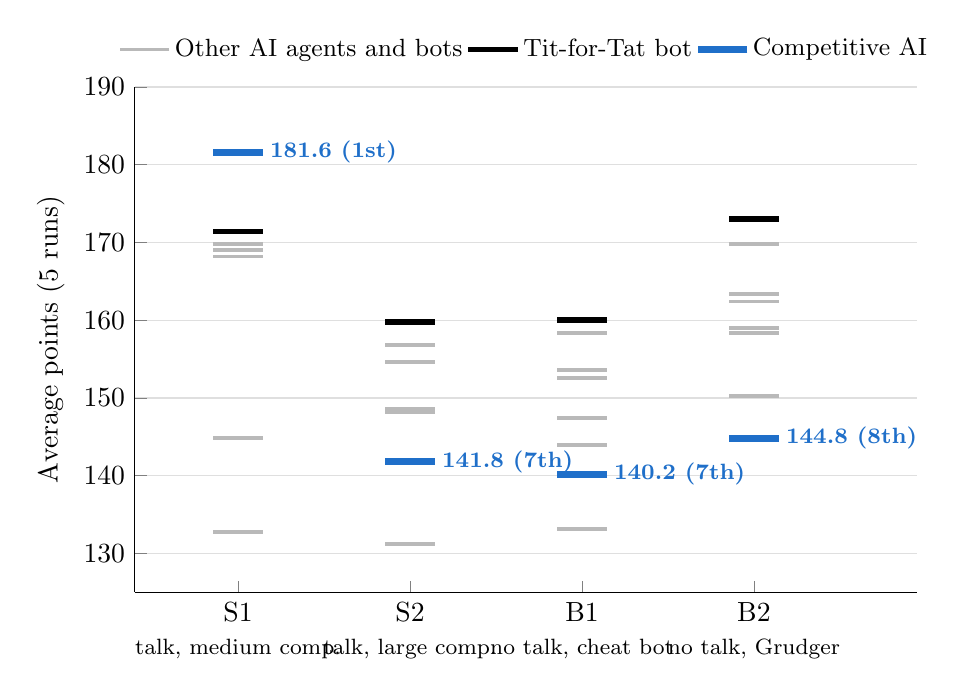
\begin{tikzpicture}
\begin{axis}[
  width=0.95\textwidth, height=8cm,
  xmin=0.4, xmax=4.95, clip=false, ymin=125, ymax=190,
  xtick={1,2,3,4},
  xticklabels={{S1\\\footnotesize talk, medium comp.},{S2\\\footnotesize talk, large comp.},{B1\\\footnotesize no talk, cheat bot},{B2\\\footnotesize no talk, Grudger}},
  xticklabel style={align=center},
  ylabel={Average points (5 runs)},
  ymajorgrids, grid style={gray!25},
  axis lines*=left,
  legend style={at={(0.5,1.03)},anchor=south,legend columns=3,draw=none,font=\small},
  legend cell align=left,
]
% Other players
\addplot[only marks, mark=-, mark size=9pt, othergray, line width=1.4pt] coordinates {
 (1,169.8) (1,169.0) (1,168.2) (1,168.2) (1,144.8) (1,132.8)
 (2,156.8) (2,154.6) (2,154.6) (2,148.6) (2,148.2) (2,131.2)
 (3,158.4) (3,153.6) (3,152.6) (3,147.4) (3,144.0) (3,133.2)
 (4,169.8) (4,163.4) (4,162.4) (4,159.0) (4,158.4) (4,150.2)};
\addlegendentry{Other AI agents and bots}
% Tit-for-Tat
\addplot[only marks, mark=-, mark size=9pt, black, line width=2pt] coordinates {
 (1,171.4) (2,159.8) (3,160.0) (4,173.0)};
\addlegendentry{Tit-for-Tat bot}
% Competitive AI
\addplot[only marks, mark=-, mark size=9pt, compblue, line width=2.6pt] coordinates {
 (1,181.6) (2,141.8) (3,140.2) (4,144.8)};
\addlegendentry{Competitive AI}
\node[compblue,anchor=west,font=\footnotesize\bfseries] at (axis cs:1.13,181.6) {181.6 (1st)};
\node[compblue,anchor=west,font=\footnotesize\bfseries] at (axis cs:2.13,141.8) {141.8 (7th)};
\node[compblue,anchor=west,font=\footnotesize\bfseries] at (axis cs:3.13,140.2) {140.2 (7th)};
\node[compblue,anchor=west,font=\footnotesize\bfseries] at (axis cs:4.13,144.8) {144.8 (8th)};
\end{axis}
\end{tikzpicture}
\caption{Average score of each player by setting. Each horizontal mark is one player. The competitive AI won only when it could talk and used a cooperate-then-betray strategy (S1); when it defected unconditionally it ranked 7th or 8th.}
\label{fig:scores}
\end{figure}

\subsection{Behaviour}

Table~\ref{tab:behaviour} summarises behaviour across all 20 tournaments.

\begin{table}[htbp]
\centering
\caption{Behavioural measures across settings. Cooperation is the range of per-setting averages; betrayals and forgiveness are pooled over all runs in which the player appeared.}
\label{tab:behaviour}
\small
\begin{tabularx}{\textwidth}{@{}lccL@{}}
\toprule
Player & Cooperation rate & Unprovoked betrayals & Forgiveness of noise \\
\midrule
Cooperative AI  & 67--82\% & 2 & 87\% (83/95) \\
Large AI        & 67--79\% & 0 & 79\% (67/85) \\
Small AI        & 66--76\% & 7 & 68\% (52/77) \\
Medium AI       & 66--80\% & 0 & 64\% (38/59) \\
Tit-for-Tat bot & 63--71\% & 0 & 0\% (0/107) \\
\addlinespace
Competitive AI  & 53\% (S1); 0\% (S2, B1, B2) & 20 (S1) & 33\% in S1 (11/33); defected every round elsewhere \\
\bottomrule
\end{tabularx}
\end{table}

\noindent The main patterns were:

\begin{enumerate}
  \item \textbf{Two competitive strategies.} In S1, the medium competitive agent cooperated about half the time, committed 20 unprovoked betrayals (19 of them alongside cooperative-sounding messages), and won 3 of 5 tournaments. In S2, the large competitive agent defected from round 1 and sent no messages, stating that it preferred not to make promises it would not keep.
  \item \textbf{Envy loses.} Whenever the competitive agent defected unconditionally (S2, B1, B2), it won 5.4--5.6 of its 7 matches on average yet scored lowest among all AI agents, because mutual defection yields 1 point per round instead of 3.
  \item \textbf{Nice and forgiving majority.} Neutral and cooperative agents almost never defected first (9 cases in 20 tournaments) and forgave 64--87\% of noise-induced defections, compared with 0\% for Tit-for-Tat.
  \item \textbf{Actions over words.} After round 1, agents cooperated with the lying cheat bot on average at most 0.8 times in 9 rounds, despite its friendly messages.
  \item \textbf{Negative externality.} With an unconditional defector present (S2, B1), the other AI agents scored roughly 10--20 points less than in S1.
  \item \textbf{Goal framing over model size.} Neutral agents of all three sizes scored within 11 points of each other in every setting, whereas the same model's behaviour changed completely under a different goal.
\end{enumerate}

\section{Follow-up Check: Opening Move and Call Batching}
\label{sec:check}

In B1 and B2 the medium competitive agent defected in every round of all 10 runs, suggesting that without messages it abandons the cooperate-then-betray strategy. However, in these settings a single model call decided round~1 for all 10 games and produced identical moves in each. The 10 runs therefore reflected one decision, not ten.

To separate the effect of messages from the effect of batching, we queried the medium competitive agent six times on a single round-1 game, each time in a fresh call. The prompts were identical except for the message rules (Table~\ref{tab:check}).

\begin{table}[htbp]
\centering
\caption{Opening moves of the medium competitive agent in fresh single-game calls.}
\label{tab:check}
\begin{tabular}{@{}lcc@{}}
\toprule
Prompt & Opening moves & Opened with C \\
\midrule
With messages (S1)    & C, D, C & 2 of 3 \\
Without messages (B)  & D, C, D & 1 of 3 \\
\bottomrule
\end{tabular}
\end{table}

All defecting openings gave the same rationale: defection can never leave the agent behind its opponent in a single round. All cooperating openings cited probing for reciprocity. The agent appears to choose between these two lines of reasoning almost at random. Messages may raise the probability of a cooperative opening, but three calls per condition cannot establish this. Methodologically, batching several games into one call makes those games non-independent and overstates the effective sample size.

\section{Discussion}

\paragraph{Goal wording is a key lever.} A single sentence of goal framing changed the same model from a reliable partner into an exploiter, a larger effect than changing model size. This suggests that the safety of multi-agent systems may depend as much on how deployers phrase objectives as on the models themselves, and that evaluations should test sensitivity to goal wording.

\paragraph{Axelrod's principles transfer to LLM agents.} Nice, forgiving and non-envious behaviour performed well; relative-payoff (envious) objectives won matches but lost tournaments. A one-line Tit-for-Tat rule was the most robust player.

\paragraph{Forgiveness is exploitable.} High forgiveness keeps cooperation alive under noise, but a strategic agent can disguise deliberate defections as accidents. Robust agents may need to remain forgiving while tracking patterns of repeated ``accidents''.

\paragraph{Cheap talk is double-edged.} Messages alone did not sustain deception: no agent kept trusting the lying bot, whose actions and reputation contradicted its words. Yet messages accompanied the most successful exploitation in S1. Reputation and verifiable track records may matter more than promises in agent ecosystems.

\paragraph{Aggressive agents impose costs on everyone.} A single unconditional defector reduced every other player's score, indicating that a small number of aggressive agents could degrade outcomes in open multi-agent networks.

\section{Limitations}

\begin{itemize}
  \item \textbf{Sample size.} Five runs per setting provide early signals, not statistical evidence; 20--30 runs per setting would be needed.
  \item \textbf{Mixed querying method.} Per-game and batched calls were mixed across rounds and settings; batching introduces dependence between games.
  \item \textbf{Single model family.} All agents were Claude models; other model families may behave differently.
  \item \textbf{Short horizon and fixed prompts.} Matches lasted 10 rounds, and only one wording of each goal and of the rules was tested.
  \item \textbf{One information leak.} In one round, an agent saw other players' answer files after submitting its own; instructions were tightened afterwards.
\end{itemize}

\section{Future Work}

The most informative next step is inexpensive: estimate the competitive agent's probability of a cooperative opening, with and without messages, using on the order of 100 fresh single-game calls per condition. Beyond this, we plan: (i) a clean replication of S1, S2 and B with per-game calls and 20--30 runs per setting; (ii) a control setting without a competitive agent; (iii) an all-AI society with one competitive agent; (iv) a goal-wording study comparing ``win overall'', ``beat each opponent'' and ``earn the most'' across model sizes; (v) an evolutionary variant in which low scorers adopt the top scorer's goal over several generations; and (vi) comparison with other model families, including open-weight models.

\section{Conclusion}

In an Axelrod-style tournament, LLM agents with neutral or cooperative goals behaved much like Axelrod's successful strategies: nice, forgiving and resistant to deceptive talk. A competitive goal framing produced either successful deceptive exploitation or self-defeating unconditional defection. Goal wording mattered more than model size, and a single aggressive agent harmed the whole group. These pilot results motivate larger, methodologically uniform studies of how AI agents will treat each other.

\section*{AI Assistance Statement}
The research idea, questions and study design are the author's. AI tools (Claude, by Anthropic) were used to implement the game software, run the simulations, analyse the logs and draft this manuscript. The AI players in the tournaments were also Claude models, as described in Section~2. All game logs, prompts, model responses and code are available from the author on request.

\begin{thebibliography}{3}
\bibitem{axelrod1980}
R.~Axelrod.
\newblock Effective choice in the Prisoner's Dilemma.
\newblock \emph{Journal of Conflict Resolution}, 24(1):3--25, 1980.

\bibitem{axelrod1981}
R.~Axelrod and W.~D. Hamilton.
\newblock The evolution of cooperation.
\newblock \emph{Science}, 211(4489):1390--1396, 1981.

\bibitem{axelrod1984}
R.~Axelrod.
\newblock \emph{The Evolution of Cooperation}.
\newblock Basic Books, New York, 1984.
\end{thebibliography}

\appendix
\section{Full Score Table}
\label{app:scores}

\begin{table}[htbp]
\centering
\caption{Average points per player (5 runs per setting); rank in parentheses. Scores were recomputed from raw move logs.}
\small
\begin{tabular}{@{}lcccc@{}}
\toprule
Player & S1 & S2 & B1 & B2 \\
\midrule
Competitive AI    & \textbf{181.6} (1) & 141.8 (7) & 140.2 (7) & 144.8 (8) \\
Tit-for-Tat bot   & 171.4 (2) & \textbf{159.8} (1) & \textbf{160.0} (1) & \textbf{173.0} (1) \\
Large AI          & 169.8 (3) & 156.8 (2) & 158.4 (2) & 163.4 (3) \\
Small AI          & 169.0 (4) & 154.6 (3) & 152.6 (4) & 159.0 (5) \\
Medium AI         & 168.2 (5) & 148.6 (5) & 147.4 (5) & 158.4 (6) \\
Cooperative AI    & 168.2 (5) & 154.6 (3) & 153.6 (3) & 162.4 (4) \\
Random bot        & 144.8 (7) & 148.2 (6) & 144.0 (6) & 150.2 (7) \\
Cheat bot         & 132.8 (8) & 131.2 (8) & 133.2 (8) & --- \\
Grudger bot       & --- & --- & --- & 169.8 (2) \\
\bottomrule
\end{tabular}
\end{table}

\noindent In S2 the competitive AI was the large model and the cooperative AI the small model; in all other settings both were the medium model.

\end{document}
